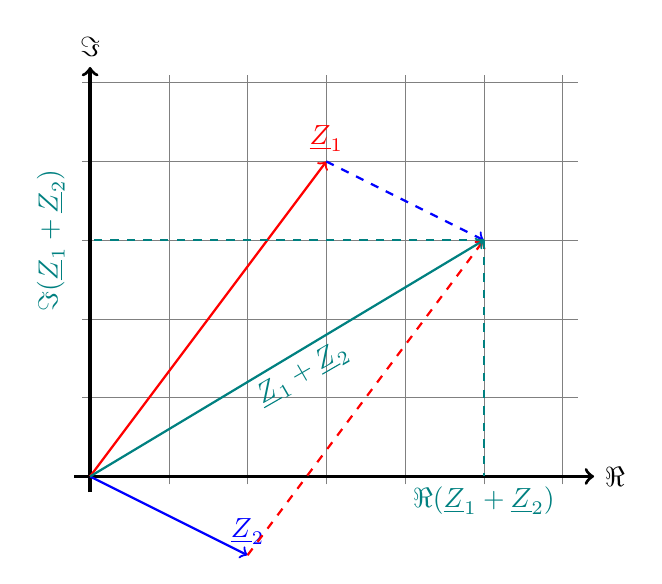
\begin{tikzpicture}
    \draw (0,0) coordinate (K);
    \draw[very thin,gray] (-0.1,-0.1) grid (6.2,5.1);
    \draw[->, very thick] (-0.2,0) -- (6.4,0) node[right] {$\Re$};
    \draw[->, very thick] (0,-0.2) -- (0,5.2) node[above] {$\Im$};
    \draw[->, thick, red] (0,0) -- (3,4) node[above] {$\underline{Z}_\mathrm{1}$};
    \draw[->, thick, blue] (0,0) -- (2,-1) node[above] {$\underline{Z}_\mathrm{2}$};


    \draw[->, dashed, thick, blue] (3,4) -- (5,3) ;
    \draw[->, dashed, thick, red] (2,-1) -- (5,3) ;


    \draw[->, thick, teal] (0,0) -- (5,3);
    \draw(2.7,1.3) node [teal, rotate=30] {$\underline{Z}_\mathrm{1}+\underline{Z}_\mathrm{2}$};
    \draw[dashed, thick, teal] (5,3) -- (0,3)
    (-0.5,3) node[rotate=90] {$\Im(\underline{Z}_\mathrm{1}+\underline{Z}_\mathrm{2}$)};
    \draw[dashed, thick, teal] (5,3) -- (5,0) node[below] {$\Re(\underline{Z}_\mathrm{1}+\underline{Z}_\mathrm{2}$)};
\end{tikzpicture}\\